%! suppress = EscapeUnderscore
Up to this point in all feedforward and convolutional neural networks we have developed, the size of the input was
always fixed, such as fixed size images to convolutional neural networks for image classification and fixed sized
window of words in Word2vec models. \v

Further, each input to the network was independent of the previous or future inputs. For example, the computations,
outputs and decisions for two successive images are completely independent of each other, and each word prediction
does not depend on the previous prediction. \v

However, in many applications the input is not of a fixed size. On top of that, successive inputs may not be
independent of each other.

\be
For example, consider the task of autocompletion. Given the first character ``d'' you want to predict the next
character ``e'' and so on. In this example successive inputs are no longer independent (while predicting ``e''
you would want to know what the previous input was in addition to the current input) and the length of the inputs and
the number of predictions you need to make is not fixed (for example, ``learn'', ``deep'', ``machine'' have different
number of characters).

\vspace{-10pt}
\fig{rnn0}{0.44}
\ee

These kind of problems are known as ``sequence learning'', because we need to look at a sequence of (dependent)
inputs and produce an output (or outputs).

\bd[Sequence Learning]
\textbf{Sequence learning} is a type of supervised machine learning task where a model is expected to predict the next
value for an input sequence of values.
\ed

Depending on the nature of the sequential problem we might end up having different kind of problems.
\bit
\item \textbf{One To One}: Both input and output are fixed size (standard feedforward neural network).
\item \textbf{One To Many}: The input is a fixed size and the output is a variable size.
\item \textbf{Many To One}: The input is a variable size and the output is a fixed size.
\item \textbf{Many To Many}: Both the input and the output are variable size.
\eit

\fig{rnn00}{0.75}

\section{Building A Recurrent Neural Network}

No matter the nature of the data or the category of the problem we need to develop a model able to deal with these
two problems:
\bit
\item Account for variable number of inputs.
\item Account for dependence between inputs.
\eit

Solving the first problem is easy. Our neural network has to be flexible to the input. The idea here is instead of
having just one neural network, to have a lot of, identical ones, and feed each unit of input to each one of them.

\begin{figure}[H]
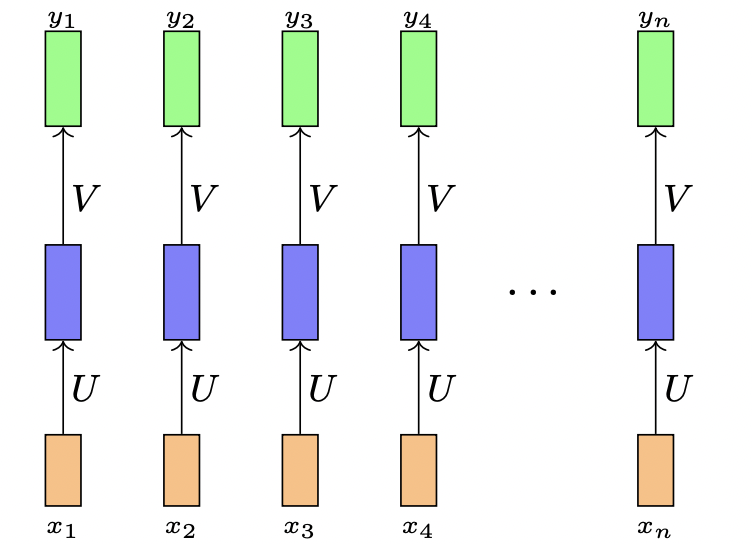
\includegraphics[scale=0.5]{rnn3}
\centering
\captionsetup{labelformat=empty}
\caption{The orange box represents the input layer, the blue box represents a generic deep feedforward neural
network (as a black box), and the green box represents the output layer. The matrix $U$ represents the input layer
parameters (both weights and biases) and the matrix $V$ represent the output layer parameters (again both weights and
biases).}
\end{figure}

Notice here, that if the functions being computed at each time-step are different, i.e.\ $\hat{y}_t = f_t(\boldsymbol{x}_{t})$,
then the network will be sensitive to the length of the sequence since it will require $f_1, f_2, \ldots,$ functions
without us knowing what the number of them should be or with no requirement to stay constant. \v

Hence, a crucial point to emphasize, is that we need to make sure that the function executed at each time-step is the
same. Or, in other words, that the parameters $U$ and $V$ are the same across all time-steps. This parameter sharing
ensures that the network becomes agnostic to the length (size) of the input, since we simply compute the same
function, with same parameters, at each time-step. We just create multiple copies of the network and execute them at
each time-step. \v

Coming to the second issue, having multiple copies of the same network, does not solve the fact the inputs are
dependent to each other. In order to deal with this problem, at time-step $t$ we will add a recurrent connection in the
network called the ``hidden state of the network at time-step $t$ $\boldsymbol{s}_{t}$''.

\bd[Hidden State]
The \textbf{hidden state} at time-step $t$ $\boldsymbol{s}_{t}$ is a $(d \times 1)$ dimensional vector encapsulating
all the information the network has seen up to time-step $t$, given by:
\bse
\boldsymbol{s}_{t} = g(U \boldsymbol{x}_{t} + W \boldsymbol{s}_{t-1}) \coloneqq RNN(\boldsymbol{s}_{t-1},
\boldsymbol{x}_{t})
\ese

with $W$ being a new, not present in standard feedforward neural networks, $(d \times d)$ matrix of parameters, used as
weights for the hidden states.
\ed

\fig{rnn4}{0.55}

\v

Before we move one, let's have a look at the hidden state equation:
\bse
\boldsymbol{s}_{t} = g(U \boldsymbol{x}_{t} + W \boldsymbol{s}_{t-1})
\ese

Let's start with the $U \boldsymbol{x}_{t}$ term. Notice that the input vector $\boldsymbol{x}_{t}$ is a $(n \times 1
)$ dimensional vector and the weight matrix $U$ is a $(d\times n)$ dimensional matrix. The function $g$, as in
feedforward neural networks, is the one responsible for the non-linearity. Since the biases are integrated in the
weights, the term $U \boldsymbol{x}_{t}$ is actually the usual activation we had in the feedforward neural networks:
\bse
\boldsymbol{a}(\boldsymbol{x}_{t} ; U) = U \boldsymbol{x}_{t}
\ese

Coming to the second, extra, term $W \boldsymbol{s}_{t-1}$ in the activation, notice that this is what produces the
dependency between the inputs, making the network able to ``remember'' the previous inputs. Notice that the formula
for the hidden states is recursive, i.e.\ the hidden state at time-step $t$ depends on the hidden state at time-step
$t-1$, and hence, the naming ``recurrent neural network''. As with $U$ and $V$, the matrix $W$ is also shared across all
time-steps in order to make sure that the network is independent of the input size. \v

Of course, for the targets of the network still holds:
\bse
\hat{y}_t = O(V \boldsymbol{s}_{t})
\ese

where $O$ is the output layer function depending on the nature of the problem under investigation. \v

This is the general architecture of a so-called ``recurrent neural network''.

\bd[Recurrent Neural Network (RNN)]
A \textbf{recurrent neural network} (\textbf{RNN}) is a class of artificial neural networks where connections between
units form a directed cycle that creates an internal hidden state of the network which allows it to exhibit dynamic temporal
behaviour.
\ed

For convenience instead of drawing multiple networks in succession, as in the previous figure, we usually draw RNNs as
follows.

\vspace{-5pt}

\fig{rnn5}{0.56}

%TODO: Bidirectional RNN

\section{Backpropagation Through Time}

As with any other neural network we have developed so far, now that the network is built we need to train it. First of
all, we need a loss function. Suppose we initialize all parameters $\theta = \{U, V, W\}$ randomly and the network
predicts the targets $\hat{y}_t$. Each network carries, the same, loss $J$ hence, we have $n$ losses of the form
$J(y_t, \hat{y}_t ; \theta)$ for each of the $n$ copies of the subnetworks. The total loss is simply the sum of the
loss over all time-steps:
\bse
J(\theta) = \sum_{t=1}^{n} J(y_t, \hat{y}_t ; \theta)
\ese

\be
Let's consider the previous example of autocompletion. Since at each time-step we want to predict either a ``d'', an
``e'', a ``p'' or a ``stop'', it's clear that we are dealing with multicalss classification problem, so we are using
Softmax as the output function. \v

After initializing all parameters $\theta = \{U, V, W\}$ randomly the network predicts the probabilities for each
target $\hat{y}_t$ and given the true targets $y_t$ we can compute the individual losses $J(y_t, \hat{y}_t ; \theta)$
and subsequently the total loss $\sum_{t=1}^{n} J(y_t, \hat{y}_t ; \theta)$.

\fig{rnn17}{0.4}
\ee

Now that we have a loss, we need an algorithm to train the model. Unsurprisingly, RNNs are trained with
backpropagation, with the only difference that now we need to update all parameters $\theta = \{U, V, W\}$ during
backpropagation. \v

For the updates we need to compute the gradients with respect to all parameters $\theta$ in order to perform the
updates in gradient descent. Since the derivative is linear, for any parameter $\theta$ holds:
\bse
\nabla_\theta J(\theta) = \sum_{t=1}^{n} \nabla_\theta J(y_t, \hat{y}_t ; \theta)
\ese

so it suffices to compute $\nabla_\theta J(y_t, \hat{y}_t ; \theta)$. \v

Starting with $V$ the derivation is exactly the same as in the usual backpropagation:
{\setlength{\jot}{5pt}
\begin{align*}
\nabla_V J(y_t, \hat{y}_t ; \theta)& = \frac{\partial J}{\partial \hat{y}_t}
\cdot \frac{\partial \hat{y}_t}{\partial (V \boldsymbol{s}_{t})} \cdot \frac{\partial (V \boldsymbol{s}_{t})}{\partial V} \\
& = \frac{\partial J}{\partial \hat{y}_t}
\cdot \frac{ \partial ( O(V \boldsymbol{s}_{t}))}{\partial (V\boldsymbol{s}_{t})} \cdot \boldsymbol{s}_{t}\\
& = \frac{\partial J}{\partial \hat{y}_t} \cdot O^\prime(V \boldsymbol{s}_{t}) \cdot \boldsymbol{s}_{t}
\end{align*}}

Moving on to $W$, things get a bit different from the usual backpropagation due to the recurrent dependency of the
network to W. More precisely: \v
\begingroup
\allowdisplaybreaks
{\setlength{\jot}{5pt}
\begin{align*}
\nabla_W J(y_t, \hat{y}_t ; \theta)& = \frac{\partial J}{\partial \hat{y}_t}
\cdot \frac{\partial \hat{y}_t}{\partial (V \boldsymbol{s}_{t})} \cdot \frac{\partial (V\boldsymbol{s}_{t})}{\partial W} \\
&= \frac{\partial J}{\partial \hat{y}_t} \cdot \frac{ \partial ( O(V\boldsymbol{s}_{t}))}{\partial (V\boldsymbol{s}_{t})}
\cdot V \cdot \frac{\partial (\boldsymbol{s}_{t})} {\partial W} \\
&= \frac{\partial J}{\partial \hat{y}_t} \cdot O^\prime(V\boldsymbol{s}_{t})
\cdot V \cdot \frac{\partial (g(U \boldsymbol{x}_{t} + W \boldsymbol{s}_{t-1}))} {\partial W} \\
&= \frac{\partial J}{\partial \hat{y}_t} \cdot O^\prime(V \boldsymbol{s}_{t})
\cdot V \cdot g^\prime(U \boldsymbol{x}_{t} + W \boldsymbol{s}_{t-1})
\cdot \frac{\partial (U\boldsymbol{x}_{t} + W \boldsymbol{s}_{t-1})} {\partial W} \\
& = \frac{\partial J}{\partial \hat{y}_t} \cdot O^\prime(V\boldsymbol{s}_{t})
\cdot V \cdot g^\prime(U \boldsymbol{x}_{t} + W \boldsymbol{s}_{t-1})
\cdot \frac{\partial (W\boldsymbol{s}_{t-1})} {\partial W} \\
& = \frac{\partial J}{\partial \hat{y}_t} \cdot O^\prime(V \boldsymbol{s}_{t})
\cdot V \cdot g^\prime(U \boldsymbol{x}_{t} + W \boldsymbol{s}_{t-1})
\cdot \left[ \boldsymbol{s}_{t-1} + W \cdot \frac{\partial(\boldsymbol{s}_{t-1})} {\partial W} \right]
\end{align*}}
\endgroup

\v

However, $\boldsymbol{s}_{t-1}$ is also a function of $W$ since:
\bse
\boldsymbol{s}_{t-1}= g(U \boldsymbol{x}_{t-1} + W \boldsymbol{s}_{t-2})
\ese

By substituting back we obtain:
{\setlength{\jot}{5pt}
\begin{align*}
\nabla_W J(y_t, \hat{y}_t ; \theta) & = \frac{\partial J}{\partial \hat{y}_t} \cdot O^\prime(V \boldsymbol{s}_{t})
\cdot V \cdot g^\prime(U \boldsymbol{x}_{t} + W \boldsymbol{s}_{t-1}) \cdot \left[ \boldsymbol{s}_{t-1} + W
\cdot \frac{\partial (g(U \boldsymbol{x}_{t-1} + W \boldsymbol{s}_{t-2}))} {\partial W} \right] \\
& = \frac{\partial J}{\partial \hat{y}_t} \cdot O^\prime(V\boldsymbol{s}_{t})
\cdot V \cdot g^\prime(U\boldsymbol{x}_{t} + W \boldsymbol{s}_{t-1})
\cdot \left[\boldsymbol{s}_{t-1} + W \cdot g^\prime (U\boldsymbol{x}_{t-1} + W \boldsymbol{s}_{t-2})
\cdot \frac{\partial (U\boldsymbol{x}_{t-1} + W \boldsymbol{s}_{t-2})} {\partial W} \right] \\
&= \frac{\partial J}{\partial \hat{y}_t} \cdot O^\prime(V\boldsymbol{s}_{t}) \cdot V
\cdot g^\prime(U\boldsymbol{x}_{t} + W \boldsymbol{s}_{t-1}) \cdot \left[\boldsymbol{s}_{t-1} + W \cdot g^\prime
(U \boldsymbol{x}_{t-1} + W \boldsymbol{s}_{t-2}) \cdot \frac{\partial (W \boldsymbol{s}_{t-2}))} {\partial W} \right] \\
&= \frac{\partial J}{\partial \hat{y}_t} \cdot O^\prime(V \boldsymbol{s}_{t}) \cdot V
\cdot g^\prime(U \boldsymbol{x}_{t} + W \boldsymbol{s}_{t-1}) \cdot \left[\boldsymbol{s}_{t-1} + W \cdot g^\prime
(U \boldsymbol{x}_{t-1} + W \boldsymbol{s}_{t-2}) \cdot \left[\boldsymbol{s}_{t-2} + W
\cdot \frac{\partial(\boldsymbol{s}_{t-2})} {\partial W} \right] \right] \\ &= \ldots
\end{align*}}

Similarly, $\boldsymbol{s}_{t-2}$ is also a function of $W$, and with this recursive way we proceed until we reach the
first network where the backpropagation is over. \v

Finally, for $\nabla_U J(y_t, \hat{y}_t ; \theta)$ we have exactly the same situation as with $W$, i.e.\ :
\begingroup
\allowdisplaybreaks
{\setlength{\jot}{5pt}
\begin{align*}
\nabla_U J(y_t, \hat{y}_t ; \theta)& = \frac{\partial J}{\partial \hat{y}_t}
\cdot \frac{\partial \hat{y}_t}{\partial (V \boldsymbol{s}_{t})} \cdot \frac{\partial (V \boldsymbol{s}_{t})}{\partial U} \\
&= \frac{\partial J}{\partial \hat{y}_t} \cdot \frac{ \partial ( O(V\boldsymbol{s}_{t}))}{\partial (V\boldsymbol{s}_{t})}
\cdot V \cdot \frac{\partial (\boldsymbol{s}_{t})}{\partial U} \\
&= \frac{\partial J}{\partial \hat{y}_t} \cdot O^\prime(V \boldsymbol{s}_{t}) \cdot V
\cdot \frac{\partial (g(U \boldsymbol{x}_{t} + W \boldsymbol{s}_{t-1}))} {\partial U} \\
&= \frac{\partial J}{\partial \hat{y}_t} \cdot O^\prime(V \boldsymbol{s}_{t}) \cdot V
\cdot g^\prime(U \boldsymbol{x}_{t} + W \boldsymbol{s}_{t-1})
\cdot \frac{\partial (U \boldsymbol{x}_{t} + W \boldsymbol{s}_{t-1})} {\partial U} \\
& = \frac{\partial J}{\partial \hat{y}_t} \cdot O^\prime(V \boldsymbol{s}_{t}) \cdot V \cdot g^\prime(U \boldsymbol{x}_{t}
+ W \boldsymbol{s}_{t-1}) \cdot \left[\boldsymbol{x_{t}}
+ W \cdot \frac{\partial(\boldsymbol{s}_{t-1})} {\partial U} \right] \\
& = \frac{\partial J}{\partial \hat{y}_t} \cdot O^\prime(V \boldsymbol{s}_{t}) \cdot V \cdot g^\prime(U \boldsymbol{x}_{t}
+ W \boldsymbol{s}_{t-1}) \cdot \left[\boldsymbol{x_{t}} + W \cdot \frac{\partial (g(U\boldsymbol{x}_{t-1}
+ W \boldsymbol{s}_{t-2}))} {\partial U}\right] \\
& = \frac{\partial J}{\partial \hat{y}_t} \cdot O^\prime(V\boldsymbol{s}_{t}) \cdot V \cdot g^\prime(U\boldsymbol{x}_{t}
+ W \boldsymbol{s}_{t-1}) \cdot \left[\boldsymbol{x_{t}} + W \cdot g^\prime (U\boldsymbol{x}_{t-1}
+ W \boldsymbol{x}_{t-2}) \cdot \frac{\partial(U \boldsymbol{x}_{t-1} + W\boldsymbol{s}_{t-2})} {\partial U} \right] \\
&= \frac{\partial J}{\partial \hat{y}_t} \cdot O^\prime(V\boldsymbol{s}_{t}) \cdot V \cdot g^\prime(U\boldsymbol{x}_{t}
+ W \boldsymbol{s}_{t-1}) \cdot \left[\boldsymbol{x_{t}} + W \cdot g^\prime (U\boldsymbol{x}_{t-1}
+ W \boldsymbol{s}_{t-2}) \cdot \left[\boldsymbol{x}_{t-1}
+ W \cdot \frac{\partial(\boldsymbol{s}_{t-2})} {\partial U} \right] \right] \\
& = \ldots
\end{align*}}
\endgroup

Hence, we have computed the gradients for all parameters $\theta = \{U, V, W\}$, and we can now perform the updates in
gradient descent. The main difference with the usual backpropagation is that in RNNs beside of just backpropagating
back to the network we also backpropagate over all previous time-steps (i.e.\ back in time). For this reason we call
this backpropagation method ``backpropagation through time''.

\bd[Backpropagation Through Time (BPTT)]
\textbf{Backpropagation through time} (\textbf{BPTT}) is an application of the backpropagation algorithm to a recurrent
neural network architecture, used to calculate the gradient of the loss function of the neural network with respect to
the weights of the network.
\ed

\subsection{Problems Of Backpropagation Through Time}

Backpropagation through time carries two major drawbacks. The first one is that due to its recursive nature it is
computationally very expensive. However, the second and most important one is the one that makes backpropagation
through time also a bit useless. Notice that the gradients of both $W$ and $U$ include the weights $W$ themselves
multiple times. If we expand the formulas, and we do the calculation we will find out that the formulas actually
contain a lot of increasing powers of $W$, i.e.\ : $W, W^2, W^3, \ldots, W^n$. This has as a result the following:
\bit
\item \textbf{Exploding Gradients} If $W > 1$ then $W^i \to \infty, \text{as } i \to n$ which has as a result for
the backpropagation through time to have bigger and bigger steps as time passes having as a result non-convergence to
the optimal point.
\item \textbf{Vanishing Gradients}: If $W < 1$ then $W^i \to 0, \text{as } i \to n$ which has as a result the terms
due to further back time-steps to have smaller and smaller gradients hence, to contribute less and less. This adds
bias parameter to the model since it captures only short term dependencies. For vanishing gradients we have the
following solutions.
\eit

In general exploding gradients it is not such a big problem since we have the following solution:
\bit
\item \textbf{Gradient Clipping}: In gradient descent we are mainly interested in the direction of the gradient and
not the magnitude of it. Hence, just by keeping the direction the same, we can manipulate the magnitude if it
explodes. With gradient clipping, a predetermined gradient threshold is introduced, and then gradients norms that
exceed this threshold are scaled down to match the norm. This prevents any gradient to have norm greater than the
threshold and thus the gradients are clipped. There is an introduced bias in the resulting values from the gradient,
but gradient clipping can keep things stable.
\eit

Vanishing gradients is a much more serious problem since it is not solved by gradient clipping. However, there are
many solutions to this problem one good try:
\bit
\item \textbf{ReLU Activation Function}: By using ReLU as activation function we force the gradients to be 1 since the
derivative of ReLU is 1 when $x>0$.
\item \textbf{Truncated Backpropagation Through Time}: In truncated backpropagation through time we truncate the sum
after a predetermined number of steps $\tau$. This leads to an approximation of the true gradient, simply by ignoring
higher terms of $W$.
\item \textbf{Parameter Initialization}: It is shown that by initializing weights to 1 and biases to 0 helps from
preventing the parameters to shrink to 0.
\item \textbf{Alternative Architectures}: However, the best, and most used, way of dealing with this problem is to
build more complex RNNs that are able to control what information is passed through. In what follows we will explore two
of the most heavily used allternative RNN architectures:
\bit
\item \textbf{Long Short Term Memory (LSTM)}: The LSTM architecture is designed to overcome the vanishing gradient
problem. It is the most used RNN architecture.
\item \textbf{Gated Recurrent Unit (GRU)}: The GRU architecture is a simplified version of the LSTM architecture.
It is also designed to overcome the vanishing gradient problem.
\eit
\eit

\section{Long Short Term Memory}

One of the problems of RNNs is that while sometimes we only need to look at recent information to perform the present
task, there are also cases where we need context back from the past. Due to vanishing gradients RNNs become unable to
learn to connect the information.

\bd[Long Short Term Memory (LSTM)]
\textbf{Long Short Term Memory} networks (\textbf{LSTMs}) are a special kind of RNN, capable of learning long-term
dependencies.
\ed

LSTMs were introduced by Hochreiter and Schmidhuber in 1997 and were refined and popularized by many people lately.
They work tremendously well on a large variety of problems, and are now widely used. LSTMs are explicitly designed to
avoid the long-term dependency problem. Remembering information for long periods of time is practically their default
behaviour, not something they struggle to learn! \v

Now let's try to build and LSTM step by step. Up to this point, we have computed a hidden state $\boldsymbol{s}_{t-1}$
at time-step $t - 1$, and by overloading it with new information $\boldsymbol{x}_{t}$ we compute a new hidden state
$\boldsymbol{s}_{t}$:
\bse
\boldsymbol{s}_{t} = g(U \boldsymbol{x}_{t} + W \boldsymbol{s}_{t-1})
\ese

\fig{rnn6}{0.6}

Moving on to LSTMs, we will alter the current behaviour of RNNs by making use of the so-called ``gates'' or ``cells''.

\bd[Gate / Cell]
A \textbf{gate}, or \textbf{cell}, unit is a structure that gives an RNN the capability of longer memory of past events.
\ed

Focusing on the beginning of the process at time-step $t-1$, instead of passing $\boldsymbol{s}_{t-1}$ as it is, we
want to selectively write only some portions of it to the next hidden state. In the strictest case our decisions could
be binary, but a more sensible way of doing this would be to assign a value between 0 and 1 which determines what
fraction of the current hidden state to pass on to the next hidden state. \v

Hence, we introduce a new vector $\boldsymbol{o}_{t-1}$, called the ``output gate'', which decides what fraction of each
element of $\boldsymbol{s}_{t-1}$ should be passed to the next hidden state.

\bd[Output Gate]
The \textbf{output gate} $\boldsymbol{o}_{t-1}$ is a gate that decides what fraction of each element of the previous
hidden state should be passed to the next hidden state.
\ed

Each element of $\boldsymbol{o}_{t-1}$ (which is restricted to be between 0 and 1) gets multiplied element-wise with
the corresponding element of $\boldsymbol{s}_{t-1}$ to produce the ``new'', modified input hidden state:

\bse
\boldsymbol{h}_{t-1} = \boldsymbol{s}_{t-1} \odot \boldsymbol{o}_{t-1}
\ese

\v

This process is called ``selective write''.

\bd[Selective Write]
\textbf{Selective rite} is the process of deciding what fraction of each element of the previous hidden state should be passed
to the next hidden state.
\ed

\fig{rnn7}{0.68}

As usual, we let the network learn what the appropriate $\boldsymbol{o}_{t-1}$ should be by parametrizing it. At this
point we should mention that there are many variations of the parametrized formula of $\boldsymbol{o}_{t-1}$, ending up
in different variations of LSTMs. Here we will use the most used one which is:
\bse
\boldsymbol{o}_{t-1} = \sigma(U_{\text{o}} \boldsymbol{x}_{t-1} + W_{\text{o}} \boldsymbol{h}_{t-2})
\ese

The new parameters $U_{\text{o}}, W_{\text{o}}$ need to be learned along with the existing parameters $W, U, V$. \v

Moving on, the input $\boldsymbol{x}_{t}$ enters the picture. Recall that in plain RNN we had:
\bse
\boldsymbol{s}_{t} = g(U \boldsymbol{x}_t + W \boldsymbol{s}_{t-1})
\ese

In LSTM, we will simply use $\boldsymbol{h}_{t-1}$ instead of $\boldsymbol{s}_{t-1}$ to compute the new hidden state at the
next time-step, i.e.\ :
\bse
\boldsymbol{\tilde{s}}_t = g(U \boldsymbol{x}_t + W \boldsymbol{h}_{t-1})
\ese

Notice that $W$ and $U$ are similar to the parameters we used in RNN\@.

\fig{rnn8}{0.68}

Hence, $\boldsymbol{\tilde{s}}_t$ captures all the information from the previous hidden state $\boldsymbol{h}_{t-1}$ and the
current input $\boldsymbol{x}_t $. However, we may not want to use all this new information and only selectively read
from it before constructing the new gate hidden state $\boldsymbol{s}_t$. To do this we introduce another gate called the
``input gate''.

\bd[Input Gate]
The \textbf{input gate} $\boldsymbol{i}_{t}$ is a gate that decides what fraction of each element of the new hidden state
$\boldsymbol{\tilde{s}}_t$ should be passed to the next hidden state.
\ed

The input gate follows the same structure as the output gate:
\bse
\boldsymbol{i}_{t} = \sigma(U_{\text{i}} \boldsymbol{x}_{t} + W_{\text{i}} \boldsymbol{h}_{t-1})
\ese

The new parameters $U_{\text{i}}, W_{\text{i}}$ need to be learned along with the existing parameters
$W, U, V$ and the output gate parameters $U_{\text{o}}, W_{\text{o}}$. \v

As before with the input gate, each element of the output gate $\boldsymbol{i}_{t}$ (which is again restricted to be
between 0 and 1) gets multiplied element-wise with the corresponding element of $\boldsymbol{\tilde{s}}_t$ to produce
the ``new'', modified input hidden state:
\bse
\boldsymbol{\tilde{s}}_t \odot \boldsymbol{i}_{t}
\ese

This process is called ``selective read''.

\bd[Selective Read]
\textbf{Selective read} is the process of deciding what fraction of each element of the new hidden state
$\boldsymbol{\tilde{s}}_t$ should be passed to the next hidden state.
\ed

\fig{rnn9}{0.7}

Coming to the final step we want to find a way to combine $\boldsymbol{s}_{t-1}$and $\boldsymbol{\tilde{s}}_t$ to get
the new hidden state $\boldsymbol{s}_{t}$. In order to do so, we introduce one final gate called the ``forget gate'' that we
use in order to forget some parts of $\boldsymbol{s}_{t-1}$.

\bd[Forget Gate]
The \textbf{forget gate} $\boldsymbol{f}_{t}$ is a gate that decides what fraction of each element of the previous
hidden state $\boldsymbol{s}_{t-1}$ should be passed to the next hidden state.
\ed

The forget gate follows the same structure as the input and output gates:
\bse
\boldsymbol{f}_{t} = \sigma(U_{\text{f}} \boldsymbol{x}_{t} + W_{\text{f}} \boldsymbol{h}_{t-1})
\ese

The new parameters $U_{\text{f}}, W_{\text{f}}$ need to be learned along with the existing parameters $W, U, V$ and
the output gate parameters $U_{\text{o}}, W_{\text{o}}$ and the input gate parameters $U_{\boldsymbol{i}},
W_{\boldsymbol{i}}$. \v

As with the other two gates each element of the forget gate $\boldsymbol{f}_{t} $ (which is once again restricted to be
between 0 and 1) gets multiplied element-wise with the corresponding element of $\boldsymbol{s}_{t-1}$ to produce the
final next hidden state:
\bse
\boldsymbol{s}_{t} =\boldsymbol{\tilde{s}}_t \odot \boldsymbol{i}_{t} + \boldsymbol{s}_{t-1} \odot \boldsymbol{f}_{t}
\coloneqq LSTM(\boldsymbol{s}_{t-1}, \boldsymbol{x}_{t})
\ese

This process is called ``selective forget''.

\bd[Selective Forget]
\textbf{Selective forget} is the process of deciding what fraction of each element of the previous hidden state
$\boldsymbol{s}_{t-1}$ should be passed to the next hidden state.
\ed

\fig{rnn11}{0.65}

After we have $\boldsymbol{s}_{t} $ we can start the process again for the next time-step.

\fig{rnn12}{0.6}

This is the structure of LSTM. Let's summarise all the steps once again.
\ben
\item Being at time-step $t$, from previous time-step get $\boldsymbol{h}_{t-1}$ and $\boldsymbol{s}_{t-1}$.
\item From current time-step get the input $\boldsymbol{x}_{t}$.
\item By using $\boldsymbol{h}_{t-1}$ and the input $\boldsymbol{x}_{t}$ compute $\boldsymbol{\tilde{s}}_t = g
(U\boldsymbol{x}_t + W \boldsymbol{h}_{t-1})$.
\item By defining the input gate $\boldsymbol{i}_{t} = \sigma(U_{\text{i}} \boldsymbol{x}_{t} + W_{\text{i}}
\boldsymbol{h}_{t-1})$, the forget gate $\boldsymbol{f}_{t} = \sigma (U_{\text{f}} \boldsymbol{x}_{t} +
W_{\text{f}} \boldsymbol{h}_{t-1})$, and by using $\boldsymbol{s}_{t-1}$ and $\boldsymbol{\tilde{s}}_t$ compute the
next hidden state: $\boldsymbol{s}_{t} =\boldsymbol{\tilde{s}}_t\odot \boldsymbol{i}_{t} + \boldsymbol{s}_{t-1} \odot
\boldsymbol{f}_{t}$.
\item By defining the output gate $\boldsymbol{o}_{t} = \sigma (U_{\text{o}} \boldsymbol{x}_{t} + W_{\text{o}}
\boldsymbol{h}_{t-1})$ and by using $\boldsymbol{s}_{t}$ compute $\boldsymbol{h}_{t} = \boldsymbol{s}_{t} \odot
\boldsymbol{o}_{t}$.
\item Pass $\boldsymbol{h}_{t}$ and $\boldsymbol{s}_{t}$ to the next time-step and repeat!
\een

We usually represent each cycle (steps 1 to 5) graphically as follows.

\fig{rnn14}{0.5}

And of course the final step 6 is the one that adds the recursivity. We represent each the whole LSTM graphically as
follows.

\fig{rnn15}{0.43}

Now let's try to give an intuition of what LSTM does exactly! During forward propagation the gates control the flow
of information. They prevent any irrelevant information from being written to the hidden state. Similarly, during backward
propagation they control the flow of gradients. It is easy to see that during backward pass the gradients will get
multiplied by the gate. For example, if the hidden state at time $t - 1$ did not contribute much to the hidden state at time $t$
(either because $\boldsymbol{o}_{t-1} \to 0$ or $\boldsymbol{f}_{t} \to 0$) then during backpropagation the gradients
flowing into $\boldsymbol{s}_{t-1}$ will vanish. But this kind of vanishing gradient is fine (since
$\boldsymbol{s}_{t-1}$ did not contribute to $\boldsymbol{s}_{t}$ it makes sense that we don't want to hold it
responsible for the crimes of $\boldsymbol{s}_{t}$). The key difference from RNNs is that the flow of information and
gradients is controlled by the gates which ensure that the gradients vanish only when they should (i.e.\ when
$\boldsymbol{s}_{t-1}$ didn't contribute much to $\boldsymbol{s}_{t}$). \v

Coming to how LSTMs solve the problem of vanishing gradients (when they shouldn't vanish) the most important think to
notice from the diagrams is that the newly introduced gates introduced themselves extra ``hidden'' hidden states
$\boldsymbol{\tilde{s}}$ and $\boldsymbol{h}_{t}$ which they also depend on in $\boldsymbol{s}_{t}$. In other words
there is a plethora of ways that each hidden state $\boldsymbol{s}_{t}$ ``reaches'' the loss function $J$ in the end of the
network. It suffices to find just one that does not vanish, since that way we make sure that the information will
remain in the network through backpropagation. We can show that for any given hidden state $\boldsymbol{s}_{t}$, by
following the path shown in the figure below, we can ensure that the gradient will not vanish (unless the hidden state
vanishes during forward propagation which, as we argued, then it's fine). The calculation are quite straight-forward
(simply start from the loss and by making use of the chain rule stat propagating back) and very similar to the ones
we did before for simple RNNs, so we will skip them!

\fig{rnn16}{0.43}

As we already mentioned, LSTM has many variants which include different number of gates and also different arrangement
of gates. The one which we just saw is one of the most popular variants of LSTM. Another equally popular variant of
LSTM is the Gated Recurrent Unit which we will see next.

\section{Gated Recurrent Unit}

Gated recurrent units (GRUs) are a gating mechanism in recurrent neural networks, introduced in 2014 by Kyunghyun Cho.
The GRU is like a long short-term memory (LSTM) with an output and an input gate, but has fewer parameters than
LSTM, as it lacks a forget gate. Since the structure of GRU is very similar to LSTM, let's give a summary of the
model instead of going through it step by step.

\ben
\item Being at time-step $t$, from previous time-step get $\boldsymbol{s}_{t-1}$.
\item From current time-step get the input $\boldsymbol{x}_{t}$.
\item By using $\boldsymbol{s}_{t-1}$ and the input $\boldsymbol{x}_{t}$ define the gate $\boldsymbol{o}_{t} = \sigma
(U_{\text{o}} \boldsymbol{x}_{t} + W_{\text{o}} \boldsymbol{s}_{t-1})$.
\item By using the output gate $\boldsymbol{o}_{t}$ and $\boldsymbol{s}_{t-1}$ compute $\boldsymbol{\tilde{s}}_t = g
(U\boldsymbol{x}_{t} + W (\boldsymbol{s}_{t-1} \odot \boldsymbol{o}_{t}))$.
\item By defining the input gate $\boldsymbol{i}_{t} = \sigma(U_{\text{i}} \boldsymbol{x}_{t} + W_{\text{i}}
\boldsymbol{s}_{t-1})$ and by using both $\boldsymbol{s}_{t-1}$ and $\boldsymbol{\tilde{s}}_t $ compute the next
hidden state $\boldsymbol{s}_{t} = \boldsymbol{s}_{t-1} \odot (1 - \boldsymbol{i}_{t}) + \boldsymbol{\tilde{s}}_t
\odot \boldsymbol{i}_{t} \coloneqq GRU(\boldsymbol{s}_{t-1}, \boldsymbol{x}_{t}) $.
\item Pass $\boldsymbol{s}_{t}$ to the next time-step and repeat!
\een

\section{Encoder-Decoder Model}

The encoder-decoder architecture allows for the transformation of a sequence of inputs into a sequence of outputs.
It comprises two sub-models: the ``encoder'' and the ``decoder''.

\bd[Encoder]
An \textbf{encoder} is a neural network that takes an input sequence and encodea it into a hidden state, fixed length
vector representation.
\ed

The encoder is usually a stack of several recurrent units (LSTMs or GRUs) where each accepts a single element of the
input sequence, collects information for that element, and propagates it forward through its hidden state
$\boldsymbol{h}$ (we denote the hidden states of the encoder with the letter $\boldsymbol{h}$ to distinguish them from
the hidden states of the decoder):
\bse
\boldsymbol{h}_{t} = RNN(\boldsymbol{h}_{t-1}, \boldsymbol{x}_{t})
\ese

The final hidden state $\boldsymbol{h}_T$ produced from the encoder, aims to encapsulate the information for all input
elements,and acts as the initial hidden state of the decoder.

\fig{rnn20}{0.5}

\bd[Decoder]
A \textbf{decoder} is a neural network that takes a hidden state, fixed length vector representation and converts it
into an output.
\ed

The decoder is usually a stack of several recurrent units (LSTMs or GRUs) where each accepts a hidden state from the
previous unit and produces and output as well as its own hidden state $\boldsymbol{s}$ (we denote the hidden states of
the decoder with the letter $\boldsymbol{s}$ to distinguish them from the hidden states of the encoder):
\bse
\boldsymbol{s}_{t} = RNN(\boldsymbol{s}_{t-1}, \boldsymbol{e}(y_{t-1}))
\ese

where $\boldsymbol{e}$ is an embedding layer that converts the output of the decoder $y_t$ into a vector representation
that is used as the input at time $t+1$ for the decoder. The initial input $\boldsymbol{e}(y_0)$ is a sign to the
decoder, usually denoted by $<\text{GO}>$, indicating the start of the decoding process. \v

\vspace{-10pt}
\fig{rnn21}{0.55}

\bd[Ecoder-Decoder Model]
\textbf{Encoder-Decoder} model is a neural network architecture composed of two RNNs arranged in such a way that
the first RNN encodes the input sequence into a fixed-length vector representation, and the second decodes this
representation into the target sequence.
\ed

In the encoder-decoder model, the final hidden state of the encoder $\boldsymbol{h}_{T}$ is set to the initial hidden
state of the decoder $\boldsymbol{s}_{0}$
\bse
\boldsymbol{h}_{T} = \boldsymbol{s}_{0}
\ese

\fig{rnn19}{0.5}

The encoder-decoder architecture is popular because it is effective and easy to implement. It is used for challenging
problems like machine translation, caption generation, and speech recognition. The encoder and decoder are trained
jointly and the model is trained to minimize the difference between the output sequence and the expected output
sequence. \v

The power of this model lies in the fact that it can map sequences of different lengths to each other. In other words
the inputs and outputs are not correlated and their lengths can differ. This opens a whole new range of problems
which can now be solved using such architecture.

\subsection{Attention}

The encoder-decoder model is very powerful, however it has one major drawback. The encoder is expected to encode all
information of the input sequence into a fixed length vector representation $\boldsymbol{h}_T$ that will feed to the
decoder. However, all past hidden states $\boldsymbol{h}_1$, $\boldsymbol{h}_2$, \ldots, $\boldsymbol{h}_{T-1}$ are
lost, or rather encapsulated in $\boldsymbol{h}_T$. The issue with this, is that the further in the past a hidden
state is, the less influence it has on $\boldsymbol{h}_T$, due to the fact that hidden states are computed
recursively, and the further back in time we go, the more the gradients vanish. \v

On top of that, at each time step $t$, not all the information of the input sequence is relevant to the output sequence.
In other words, by feeding just the final hidden state $\boldsymbol{h}_T$ to the decoder, we are forcing the decoder to
use the same information for each time step $t$, instead of focusing on the relevant parts of the input sequence at each
time step.

\be
For example, in machine translation, the translation of a word depends on a few words before and after it, but not on
the whole sentence or other sentences.
\ee

This is where the so-called ``attention '' comes into play, which mimicking cognitive attention.

\bd[Attention]
\textbf{Attention} is a mechanism that allows the decoder to focus on the relevant parts of the input sequence at each
time step.
\ed

The attention mechanism is usually implemented as a separate layer between the encoder and the decoder. It starts by
computing the so-called ``alignment score'' $e_{jt}$.

\bd[Alignment Score]
The \textbf{alignment score} $e_{jt}$ measures the similarity between the $t-1$ hidden state of the decoder
$\boldsymbol{s}_{t-1}$ and the $j$'th hidden state of the encoder $\boldsymbol{h}_j$:
\bse
e_{jt} = f(\boldsymbol{s}_{t-1}, \boldsymbol{h}_j)
\ese
\ed

Alignment score captures the importance of the $j$'th input for decoding the $t$'th output. There are many functions
$f$ that can be used to compute the alignment score that have been proposed in the literature. One can choose the
function $f$ that best suits the problem at hand. \v

The next step is to normalize the alignment scores to obtain the ``attention weights'' $\alpha_{jt}$.

\bd[Attention Weights]
The \textbf{attention weights} $\alpha_{jt}$ are the normalized alignment scores:
\bse
\alpha_{jt} = \frac{\exp(e_{jt})}{\sum_{k=1}^{T} \exp(e_{kt})}
\ese
\ed

The attention weights are also called ``soft'' weights, because they are normalized and can be interpreted as
probabilities. More specificaly, they denote the probability of focusing on the $j$'th inout to produce the $t$'th
output. \v

Once we have the attention weights, we can compute the ``context vector'' $\boldsymbol{c}_t$.

\bd[Context Vector]
The \textbf{context vector} $\boldsymbol{c}_t$ is the weighted sum of the encoder hidden states $\boldsymbol{h}_j$,
where the weights are the attention weights $\alpha_{jt}$:
\bse
\boldsymbol{c}_t = \sum_{j=1}^{T} \alpha_{jt} \boldsymbol{h}_j
\ese
\ed

The context vector $\boldsymbol{c}_t$ captures the relevant parts of the input sequence at time step $t$. \v

Finally, the context vector $\boldsymbol{c}_t$ is concatenated with the previous hidden state of the decoder
$\boldsymbol{s}_{t-1}$ to produce the new hidden state of the decoder $\boldsymbol{s}_t$:
\bse
\boldsymbol{s}_{t} = RNN(\boldsymbol{s}_{t-1}, [\boldsymbol{e}(y_{t-1}), \boldsymbol{c}_t])
\ese

The new hidden state $\boldsymbol{s}_t$ is then fed to the decoder to produce the output $y_t$:
\bse
y_t = O(V \boldsymbol{s}_t)
\ese

\vspace{-10pt}
\fig{rnn22}{0.65}

A question that physically arises is how such a model can be trained. The model would make a lot of sense if the true
attention weights were given during training time, so we could then minimize an attention loss on top of the usual
network loss. However, in practice it is very hard to get the true attention weights, since that would require someone
to manually annotate the inputs which contribute to every target output, which is a very hard task. \v

The solution is that we simply let the model train the attention weights itself. This is done by making the attention
weights differentiable. In other words, we let the model learn the attention weights just like it learns the other
parameters of the model. This tactic works because it is a better modeling choice which leads to a more informed
model. We are essentially asking the model to approach the problem in a better, more natural, way. Given enough data
it should be able to learn these attention weights just as humans do. \v

In practice indeed these models work better than the vanilla encoder decoder models, and the model manages to learn
how to focus on the most relevant inputs at each timestep. We can check this by plotting the attention weights as a
heatmap which shows a soft alignment between the inputs and the generated outputs.

\be
This figure shows a heatmap in a translation application. The lighter the color, the more the model focuses on that
input word to generate the output word.
\fig{rnn23}{0.42}
\ee